\documentclass[letterpaper,12pt,fleqn]{article}
\usepackage{matharticle}
\usepackage{tikz}
\pagestyle{empty}
\newcommand{\cycle}[1]{\left<#1\right>}
\newcommand{\p}{\phi}
\begin{document}
\section*{Cyclic Subgroups}

\begin{theorem}
  Let $G$ be a group and $a\in G$:
  \[\cycle{a}\le G\]
\end{theorem}

\begin{theproof}
  Assume $x\in\cycle{a}$ \\
  $\exists\,n\in\Z,x=a^n$ \\
  But by closure, $a^n=x\in G$ \\
  $\cycle{a}\subseteq G$ \\
  $\cycle{a}$ is a group under the induced operation of $G$. \\
  $\therefore\cycle{a}\le G$
\end{theproof}

\begin{corollary}
  Let $G$ be a group and $a\in G$:
  
  $\cycle{a}$ is the smallest subgroup of $G$ containing $a$.
\end{corollary}

\begin{theproof}
  Assume $H\le G$ such that $a\in H$ \\
  $\cycle{a}\le H$ \\
  $\forall\,H\le G,\cycle{a}\le H$ \\
  $\therefore\cycle{a}$ is the smallest subgroup of $G$ containing $a$.
\end{theproof}

\begin{definition}
  Let $G$ be a group and $a\in G$. $\cycle{a}$ is called the
  \emph{cyclic subgroup} of $G$ generated by $a$.

  The \emph{order} of $a$ is given by $\abs{\cycle{a}}$.
\end{definition}

\begin{example}
  $U_{12}=\{e^{i\frac{2\pi k}{12}}\mid0\le k<12\}$

  \bigskip

  \begin{minipage}[t]{3in}
    Let $a=e^{i\frac{2\pi 8}{12}}=e^{i\frac{4\pi}{3}}$

    $\cycle{a}=\{1,e^{i\frac{4\pi}{3}},e^{i\frac{8\pi}{3}}\}=U_3$

    $U_3\le U_{12}$
  \end{minipage}
  \begin{minipage}[t]{3in}
    Let $a=e^{i\frac{2\pi 6}{12}}=e^{i\pi}=-1$

    $\cycle{a}=\{1,-1\}$

    $U_2\le U_{12}$
  \end{minipage}

  \bigskip

  \begin{minipage}[t]{3in}
    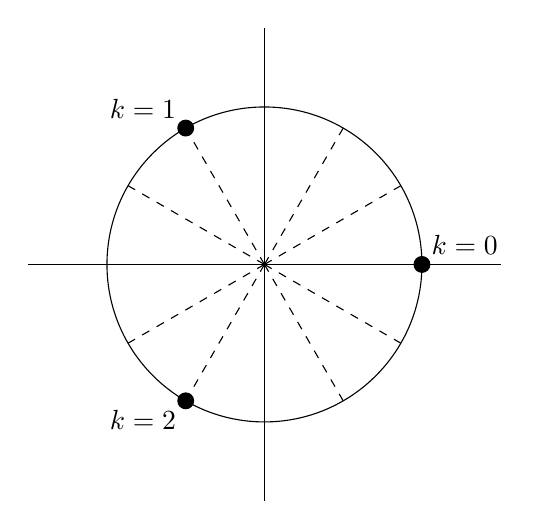
\begin{tikzpicture}
      \draw (-3,0) -- (3,0);
      \draw (0,-3) -- (0,3);
      \draw (0,0) circle [radius=2];
      \draw [dashed] (0,0) -- (1.732,1);
      \draw [dashed] (0,0) -- (1,1.732);
      \draw [dashed] (0,0) -- (-1,1.732);
      \draw [dashed] (0,0) -- (-1.732,1);
      \draw [dashed] (0,0) -- (-1.732,-1);
      \draw [dashed] (0,0) -- (-1,-1.732);
      \draw [dashed] (0,0) -- (1,-1.732);
      \draw [dashed] (0,0) -- (1.732,-1);
      \draw [fill=black] (2,0) circle [radius=0.1];
      \draw [fill=black] (-1,1.732) circle [radius=0.1];
      \draw [fill=black] (-1,-1.732) circle [radius=0.1];
      \node [above right] at (2,0) {$k=0$};
      \node [above left] at (-1,1.732) {$k=1$};
      \node [below left] at (-1,-1.732) {$k=2$};
    \end{tikzpicture}
  \end{minipage}
  \begin{minipage}[t]{3in}
    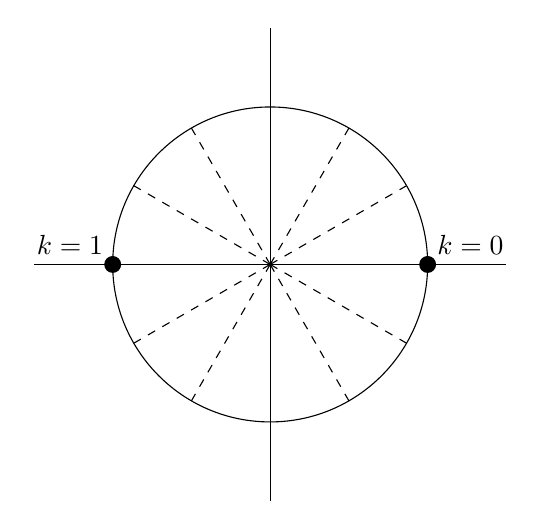
\begin{tikzpicture}
      \draw (-3,0) -- (3,0);
      \draw (0,-3) -- (0,3);
      \draw (0,0) circle [radius=2];
      \draw [dashed] (0,0) -- (1.732,1);
      \draw [dashed] (0,0) -- (1,1.732);
      \draw [dashed] (0,0) -- (-1,1.732);
      \draw [dashed] (0,0) -- (-1.732,1);
      \draw [dashed] (0,0) -- (-1.732,-1);
      \draw [dashed] (0,0) -- (-1,-1.732);
      \draw [dashed] (0,0) -- (1,-1.732);
      \draw [dashed] (0,0) -- (1.732,-1);
      \draw [fill=black] (2,0) circle [radius=0.1];
      \draw [fill=black] (-2,0) circle [radius=0.1];
      \node [above right] at (2,0) {$k=0$};
      \node [above left] at (-2,0) {$k=1$};
    \end{tikzpicture}
  \end{minipage}
\end{example}

\begin{theorem}
  Let $G$ be a group:

  $G$ has no proper, non-trivial subgroups$\implies G$ is cyclic.
\end{theorem}

\begin{theproof}
  Assume $G$ has no proper, non-trivial subgroups \\
  Assume $a\in G$ \\
  $\cycle{a}\le G$ \\
  But $\cycle{a}$ is neither trivial nor proper, so $\cycle{a}=G$ \\
  $\therefore G$ is cyclic
\end{theproof}

\begin{theorem}
  Let $G$ be cyclic. $\forall\,H\le G,H$ is cyclic.
\end{theorem}

\begin{theproof}
  $\{e\}\le G$, so AWLOG that $H\le G$ is non-trivial \\
  Let $H'=\Z_n$ or $H'=\Z$ \\
  $H\simeq H'$ \\
  Let $S=\{a\in H'\mid a\in\Z^+\}$ \\
  $1\in S$, so $S\ne\emptyset$ \\
  Let $h=\min H'$ \\
  Assume $k\in H',k\le h$ \\
  By the division algorithm: $k=qh+r$ such that $q,r\in\Z$ and $0\le r<h$ \\
  $r=k-qh\in H'$ \\
  But by the minimality of $h$, $r=0$ \\
  $k=qh$ \\
  $H'=\cycle{h}$ \\
  $H'$ is cyclic \\
  $\therefore H$ is cyclic.
\end{theproof}

\begin{theorem}
  Let $G=\cycle{a}$. Let $a^h,a^k\in G$ and $d=(h,k)$:
  \[H=\left\{\left(a^h\right)^n\left(a^k\right)^m\mid n,m\in\Z\right\}=
    \cycle{a^d}\le G\]
\end{theorem}

\begin{theproof}
  $G\simeq\Z_n$ or $G\simeq\Z$, so let $G'$ be the appropriate one \\
  Let $H'=\{mh+nk\mid m,n\in\Z$\} \\
  $H\simeq H'$ \\
  Assume $x,y\in H'$ \\
  $\exists\,m_1,n_1\in\Z,x=m_1h+n_1k$ \\
  $\exists\,m_2,n_2\in\Z,y=m_2h+n_2k$ \\
  $-y=-m_2h-n_2k\in G'$ \\
  $x-y=(m_1-m_2)h+(n_1-n_2)k\in H'$ \\
  So, by the subgroup test, $H'\le G'$ \\
  $\therefore H\le G$

  But also, $\exists\,c\in\Z,x=m_1h+n_1k=c(h,k)=cd$ \\
  So, $H'=\cycle{d}$ \\
  $\therefore H=\cycle{a^d}$
\end{theproof}

\begin{corollary}
  Let $G=\cycle{a}$. Let $a^h,a^k\in G$ and $d=(h,k)$. $\cycle{a^d}$ is the
  smallest subgroup of $G$ containing $a^h$ and $a^k$.
\end{corollary}

\begin{theproof}
  $G\simeq\Z_n$ or $G\simeq\Z$, so let $G'$ be the appropriate one \\
  Assume $H\le G'$ \\
  Assume $h,k\in H$ \\
  $\cycle{d}=\{mh+nk\mid m,n\in\Z\}\le H$ \\
  Thus, $d\in H$ \\
  $h=1\cdot h+0\cdot k\in\cycle{d}$ \\
  $k=0\cdot h+1\cdot k\in\cycle{d}$ \\
  But $\cycle{d}$ is the smallest subgroup of $H$ containing $d$ \\
  So $\cycle{d}$ is also the smallest subgroup of $H$ containing $h$ and $k$ \\
  But since $H\le G'$, $\cycle{d}$ is the smallest subgroup of $G'$ containing
  $h$ and $k$ \\
  $\therefore \cycle{a^d}$ is the smallest subgroup of $G$ containing $a^h$
  and $a^k$.
\end{theproof}

\begin{example}
  $9,15\in\Z_{24}$ and $(9,15)=3$

  $\cycle{3}=\{0,3,6,9,12,15,18,21\}$

  $\cycle{3}$ is the smallest subgroup of $\Z_{24}$ containing $9$ and $15$
\end{example}
\end{document}
